
%!TEX program = xelatex
\documentclass[letterpaper,12pt]{exam}
\usepackage{../videoNotes}
\usepackage{xcolor}
\usepackage[dvipsnames]{xcolor}
\usepackage{soul}

\newcommand{\unit}{Unit 00}
\pagestyle{headandfoot}
\firstpageheader{CSC 264 \semester\ \  \unit}{}{Name: $\rule{6cm}{0.15mm}$}
\runningheader{CSC 264 \semester}{\unit}{Page \thepage\ of \numpages}
\firstpagefooter{}{}{}
\runningfooter{}{}{}



\begin{document}
\section*{\unit\_000 -- First Assembly Program} 
\par{\fontfamily{qzc}\selectfont\textbf{Video Length 33:00}}
\begin{questions}

\begin{samepage}
    \question What symbols are used to mark a multi-line comment in the `as` assembler?
    \vspace{5mm}
\end{samepage}

\begin{samepage}
    \question What is the name of the section of the program that holds items that look like variables?  (Hint: it starts with a period.)
    \vspace{5mm}
\end{samepage}

\begin{samepage}
    \question What is the name of the section of the program that holds the executable code? (Hint: it also starts with a period.)
    \vspace{5mm}
\end{samepage}

\begin{samepage}
    \question What symbol is used to indicate that the remainder of the line is a comment?
    \vspace{5mm}

\begin{samepage}
    \question The last three lines of the program do not have comment.  Write reasonable comments for each of the lines.
    \begin{Large}
    \begin{verbatim}
movq $60, %rax

movq sum, %rdi
      
syscall
    \end{verbatim}
    \end{Large}
    \vspace{5mm}
\end{samepage}
\end{samepage}
\hrule %End of section
%----------------------------------

\section*{\unit\_010 -- About Assembly}
\par{\fontfamily{qzc}\selectfont\textbf{Video Length 8:27}}
\begin{samepage}
    \question  Is the main purpose of this course to teach you how to write programs in Assembly Language?  Explain your answer.
    \vspace{25mm}
\end{samepage}

\begin{samepage}
    \question 
    \vspace{5mm}
\end{samepage}

\par
\rule{0.5\textwidth}{.4pt} %End of section
%----------------------------------
\section*{\unit\_015 -- A Bit of History}
\par{\fontfamily{qzc}\selectfont\textbf{Video Length 20:30}}
\begin{samepage}
    \question How many bits of data were needed to represent a single decimal digit using the methods used to tablulate the US census inn 1890?
    \vspace{20mm}  Explain why it took that many bits.
\end{samepage}

\begin{samepage}
    \question How many bits are needed to represnt a single decimal diit using Binary Coded Decimal (BCD)
    \vspace{5mm}
\end{samepage}
\begin{samepage}
    \question Why was BCD inefficient?  
    \vspace{5mm}
\end{samepage}
\begin{samepage}
    \question What is the relationship between an electrical relay switch and a bit?
    \vspace{10mm}
\end{samepage}

\begin{samepage}
    \question Relays were replaced by \_\_\_\_\_\_\_\_ tubes which were in turn replaced by \rule{2cm}{0.15mm}.  Later, many transistors and other electrical components were printed on single pieces of silicone to create \rule{2cm}{0.15mm} circuits
    \vspace{5mm}
\end{samepage}
\par
\begin{samepage}
    \question How is the speed of computers related to the physical size of the CPU?
    \vspace{5mm}
\end{samepage}
\par
\begin{samepage}
    \question What is a microprocessor?
    \vspace{5mm}
\end{samepage}
\par

\rule{0.5\textwidth}{.4pt} %End of section
 
\section*{\unit\_020 -- Computer Systems}
\par{\fontfamily{qzc}\selectfont\textbf{Video Length 12:53}}
\begin{samepage}
    \question Who is generally credited with designing the basic architecture of modern computer systems?
    \vspace{5mm}
\end{samepage}
\par

\pagebreak
\begin{samepage}
    \question What are the three main components of the CPU of a CPU?
    
    \vspace{5mm}
    \begin{Large}
         1. \rule{2cm}{0.15mm}  2. \rule{2cm}{0.15mm}  3. \rule{4cm}{0.15mm}
    \end{Large}
\end{samepage}
\par
 \begin{samepage}
     \question What are registers? (You do not need to list specific registers)
     \vspace{5mm}
 \end{samepage}
 \par
 \begin{samepage}
     \question What type of arithmetic is used by the ALU?
     \vspace{5mm}
 \end{samepage}
 \par
   
 \begin{samepage}
     \question What two things are kept in Main Memory or Primary Storage?
     \vspace{5mm}
 \end{samepage}
 \par
 \begin{samepage}
     \question What unpopular opinion makes VonNeuman a controversial figure?
     \vspace{5mm}
 \end{samepage}
 \par
  \begin{samepage}
      \question Does a CPU need to be on a single chip of silicone?
      \vspace{5mm}
  \end{samepage}
  \par
   \begin{samepage}
       \question In old movies and TV shows, CPUs had lots of blinking lights.  What did the blinking lights represent?
       \vspace{5mm}
   \end{samepage}
   \par
   \begin{samepage}
       \question What is a bus?
       \vspace{5mm}
   \end{samepage}
   \par
\section*{\unit\_030 -- Computer architecture}
\par{\fontfamily{qzc}\selectfont\textbf{Video Length 8:13}}
\begin{samepage}
    \question In general terms, what does "Computer Architecture" mean?
    \vspace{5mm}
\end{samepage}
\begin{samepage}
    \question What is the specific computer architecture we will be studying this semester?
    \vspace{5mm}
ar
\end{samepage}
\begin{samepage}
    \question How wide were the registers on 8086 processors
    \vspace{5mm}
\end{samepage}
\par
\begin{samepage}
    \question How wide are the registers on 80386 processors? (Oops, I did not say 80386 in the video, so I will answer this one for you.)
    \par  
    \textcolor{blue}{\LARGE 32 bits}
    
   
\end{samepage}
\par 
\begin{samepage}
    \question How wide are the registers on x86-64 processors? (Yes, it is obvious)
    \vspace{5mm}
\end{samepage}

\begin{samepage}
    \question How are ARM processors different from x86 processors?
    \vspace{5mm}
\end{samepage}
\par
\begin{samepage}
    \question What is "Instruction Set Architecture? Do all CPUs share the same ISA?
    \vspace{15mm}
\end{samepage}
\par

\rule{0.5\textwidth}{.4pt} %End of section

\section*{\unit\_040 -- Machine Language}
\par{\fontfamily{qzc}\selectfont\textbf{Video Length 5:40}}
\begin{samepage}
    \question The assembly language program translates assembly language into \rule{3cm}{0.15mm} language.
    \vspace{5mm}
\end{samepage}
\par

NOTE:  (Not a question).  The program I wrote for the first video is in 64-bit assembler.  When i made this 040 video, I wanted the machine code to be neat in the listing.  I did not like how every line of machine code in 64-bit assembly takes two lines, with the second line being 000000000.  So I sort of cheated and wrote this program using only 16-bit assembler.  In the first program, I used the %rax register.  The "r" indicates it is 64-bit.  In the code I wrote for the 040 video, I used the %ax register, which is the 
lower 16 bits of the %rax register.  The program still works fine on a 64-bit CPU, but it looks nicer when I make a listing.  

\begin{samepage}
    \question What is the relationship between hexadecimal and binary?
    \vspace{5mm}
\end{samepage}
\par
 \begin{samepage}
     \question In the 000 video, I had the following line of code:

     \begin{verbatim}
      movq sum, %rdi       
     \end{verbatim}
     In this video, I wrote the equivalent line of code as:
     \begin{verbatim}
        mov $7, %di
        \end{verbatim}
        Explain the differences between these two lines of code.
     \vspace{5mm}
 \end{samepage}
 \par
  

\rule{0.5\textwidth}{.4pt} %End of section
%----------------------------------
\section*{\unit\_050 -- Computer Languages}
\par{\fontfamily{qzc}\selectfont\textbf{Video Length 5:28}}
\begin{samepage}
    \question How are high-level languages different from low-level languages?
    \vspace{5mm}
\end{samepage}
\par
\begin{samepage}
    \question The PDP-11 had a row of switches.  What did each switch represent?
    \vspace{5mm}
\end{samepage}
\rule{0.5\textwidth}{.4pt} %End of section
%----------------------------------


\section*{\unit\_060 -- Language Translators}
\par{\fontfamily{qzc}\selectfont\textbf{Video Length 8:00}}
\begin{samepage}
    \question I C a compiled language or an interpreted language?
    \vspace{5mm}
\end{samepage}
\par
\begin{samepage}
    \question 
    \vspace{5mm}
\end{samepage}
\par
 \begin{samepage}
     \question 
     \vspace{5mm}
 \end{samepage}
 \begin{samepage}
     \question What is the linux command that prints a program's exit code or error code.
     \vspace{5mm}
 \end{samepage}
 \par
  \begin{samepage}
      \question Is Python a compile language or an interpreted language?
      \vspace{5mm}
  \end{samepage}
  \par
   \begin{samepage}
       \question Is assembler more like a compiled language or an interpreted language?
       \vspace{5mm}
   \end{samepage}
   \par
    
\section*{\unit\_070 -- Assembler}
\par{\fontfamily{qzc}\selectfont\textbf{Video Length 7:58}}
\begin{samepage}
    \question What are the two main dialects of assemblers used for x86 assemblers?  Which are we using this semester? 
    \vspace{5mm}
\end{samepage}
\begin{samepage}
    \question Many assembly language instructions use two operands.  What order do GAS assemblers use?
    \vspace{5mm}
\end{samepage}

\begin{samepage}
     \question We assemble assembly language into machine code.  Can the process be reversed?  When would we want to reverse the process?
     \vspace{5mm}
 \end{samepage}
 

 \rule{0.5\textwidth}{.4pt} %End of section
\section*{\unit\_080 -- Generations of Programming languages}
\par{\fontfamily{qzc}\selectfont\textbf{Video Length 15:08}}
\begin{samepage}
    \question How many bits were in a register 8086 processors?  
    \vspace{5mm}
\end{samepage}
\begin{samepage}
    \question The 8086 could only address 1MB of memory.  Why was it limited to 1MB? (Hint: How many bits were in the Address Bus?)
    \vspace{5mm}
\end{samepage}
\par
\begin{samepage}
    \question What was the 8087 coprocessor used for?
    \vspace{5mm}
\end{samepage}


  \begin{samepage}
      \question How many bits were in the 80386 processor? \rule{1cm}{0.15mm}
        \vspace{5mm}
      \par Was the eax register available on the 80386? \rule{1cm}{0.15mm}
       \vspace{5mm}
      \par Was the rax register available on the 80386? \rule{1cm}{0.15mm}
  \end{samepage}
\begin{samepage}
    \question What is a "core?"
    \vspace{5mm}
\end{samepage}
\par
 \begin{samepage}
     \question To what extent does an x86-64 programmer need to be aware of the history of old processors?
     \vspace{5mm}
 \end{samepage}
 \par
  \section*{\unit\_100 -- Installing Software}
  \par{\fontfamily{qzc}\selectfont\textbf{Video Length 15:18}}
  \begin{samepage}
      \question If you want to run Linux for this semester, what would you need to consider for the minimum hardware requirement?

      \vspace{5mm}
  \end{samepage}
\begin{samepage}
    \question What is Windows Subsystem for Linux (WSL)?
    \vspace{5mm}
\end{samepage}
\par
 \begin{samepage}
     \question What is Fedora with KDE Plasma
     \vspace{5mm}
 \end{samepage}
 \par
  \begin{samepage}
      \question What is "kate?"
      \vspace{5mm}
  \end{samepage}
  \par
   \section*{\unit\_110 -- Simple Program}
   \par{\fontfamily{qzc}\selectfont\textbf{Video Length 8:24}}
   Note:  You do not need to watch this video.  You have already seen most of this program.  You may want to watch it if you have trouble getting the first assignment to work.
   
   \rule{0.5\textwidth}{.4pt} %End of section
   %----------------------------------
  \rule{0.5\textwidth}{.4pt} %End of section
  %----------------------------------
 

  %%%%%%%%%%%%%%%%%%%%%%%%%%%%%%%%%%%%%%%%%%%%%%%%%%%%%
\begin{center}
    \rule{0.5\textwidth}{.4pt}
\end{center}
Do you have any questions or concerns? Please write any lingering questions you have here.

%----------------------------------
\end{questions}
%footer
\vfill
\begin{center}
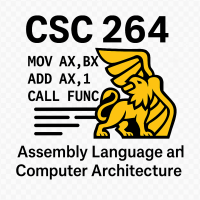
\includegraphics{../csc264Logo}
\end{center}
\end{document} 